\chapter{Aplicação do \textit{Framework}}

Neste capítulo são apresentados os resultados de cada \textit{sprint} executada nos projetos selecionados para análise. Adicionalmente, uma breve percepção é apresentada acerca dos resultados obtidos, bem como relato do que foi preciso aperfeiçoar no \textit{framework}.

\section{\textit{Sprint} 1 - Portal da Transparência do Distrito Federal}

A \textit{Sprint} 1 do projeto do portal foi executada com êxito. Todas as funcionalidades foram entregues. É válido ressaltar também que os testes unitários foram devidamente implementados para todos os componentes que sofreram alterações e também, as inspeções foram realizadas. Contudo, a equipe do projeto protelou as atividades de verificação, tornando a finalização da \textit{sprint} mais onerosa.

As tabelas a seguir exibem um resumo das métricas coletadas para as camadas de \textit{frontend} e \textit{backend}.

\begin{table}[h]
\centering
\begin{tabular}{ | m{8cm} | m{8cm} | } 
\hline
Número de Defeitos & 4 \\ 
\hline
Taxa de Acertos por Linha de Código & 3 \\ 
\hline
\end{tabular}
\caption{Tabela Resumo - Métricas \textit{Sprint} 1 - Portal da Transparência (\textit{Frontend})}\label{table:1}
\end{table}

\begin{table}[h]
\centering
\begin{tabular}{ | m{8cm} | m{8cm} | } 
\hline
Número de Defeitos & 3 \\ 
\hline
Taxa de Acertos por Linha de Código & 2 \\ 
\hline
\end{tabular}
\caption{Tabela Resumo - Métricas \textit{Sprint} 1 - Portal da Transparência (\textit{Backend})}\label{table:1}
\end{table}

A partir dos dados exibidos pelas tabelas acima, considerando somente os novos trechos de códigos produzidos e os módulos alterados, as inspeções foram capazes de identificar 4 defeitos na camada \textit{frontend} e 3 defeitos na camada \textit{backend}. De fato, por mais que os desenvolvedores da equipe estivessem implementando de forma concisa, ainda foi possível contemplar defeitos no código. Ao final da \textit{sprint}, todos os defeitos foram corrigidos antes da mesclagem final.

Com relação à taxa de acertos por linha de código, a suíte de testes elaborada foi capaz de exercitar, em média, 3 vezes os trechos de código sob teste na camada \textit{frontend} e 2 vezes os trechos de código sob teste na camada \textit{backend}. Ao final da \textit{sprint} foi possível contemplar um percentual total de cobertura igual a 15,43\% na camada \textit{frontend} e 22,10\% na camada \textit{backend}.

Com relação à camada \textit{backend}, calculou-se o índice de manutenibilidade para todos os componentes alterados. A tabela a seguir exibe estes dados, indicando a classe com o seu respectivo índice calculado.

\begin{table}[h]
\centering
\begin{tabular}{ | m{10cm} | m{6cm} | } 
\hline
Empresa Punida - \textit{Model} & 95,12 \\ 
\hline
Empresa Punida - \textit{Controller} & 94,99 \\ 
\hline
Servidores - \textit{Controller} & 49,31 \\ 
\hline
Remuneração - \textit{Controller} & 74,51 \\ 
\hline
Empresa Punida Relatório - \textit{Service} & 84,82 \\
\hline
\end{tabular}
\caption{Índice de Manutenibilidade \textit{Sprint} 1 - Portal da Transparência (\textit{Backend})}\label{table:1}
\end{table}

Foi possível perceber um valor baixo do índice para a classe \textit{ServidoresController} tendo em vista os valores que as demais classes atingiram. Contudo, é um valor aceitável de acordo com os parâmetros da \textit{Microsoft} e indica a direção para futuros esforços em refatoração.

Com relação ao número de falhas identificadas pela área de negócio, nada foi reportado. Este aspecto indica que uma verificação concisa possui forte impacto na qualidade do produto entregue.

Por fim, tem-se o percentual obtido para as respostas relacionadas ao questionário de verificação da satisfação dos desenvolvedores ao utilizarem o \textit{framework}. Foi possível perceber que a equipe de desenvolvimento do portal apresentou boa aceitação quanto ao uso do \textit{framework}. Em linhas gerais, as inspeções e a forma de implementar testes unitários foram bem vistas pelos desenvolvedores. Ainda assim, as práticas propostas, segundo os desenvolvedores da equipe, se mostratam onerosas em contextos de equipes pequenas (até 3 desenvolvedores). As figuras a seguir exibem esses percentuais.

\begin{figure}[!h]
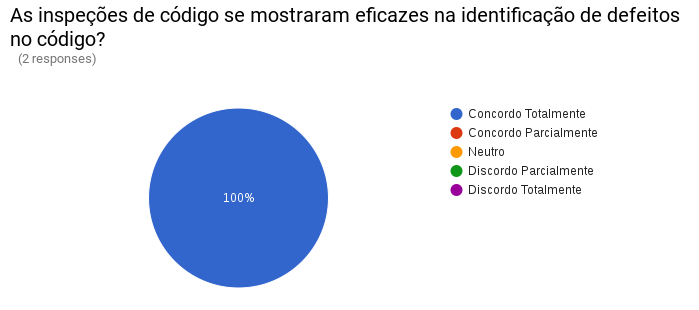
\includegraphics[width=\textwidth]{figuras/s1p.png}
\caption{Questão 1 - Satisfação dos Desenvolvedores - \textit{Sprint} 1 Portal}
\end{figure}

\begin{figure}[!h]
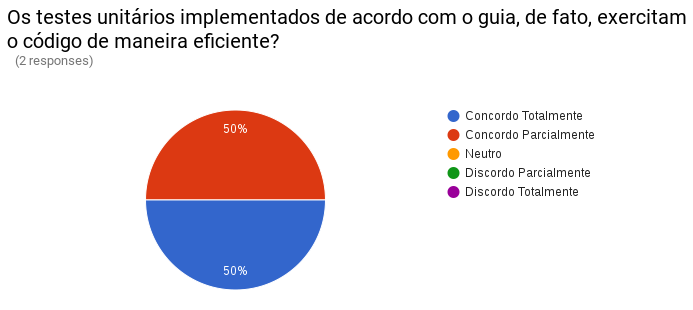
\includegraphics[width=\textwidth]{figuras/s2p.png}
\caption{Questão 2 - Satisfação dos Desenvolvedores - \textit{Sprint} 1 Portal}
\end{figure}

\begin{figure}[!h]
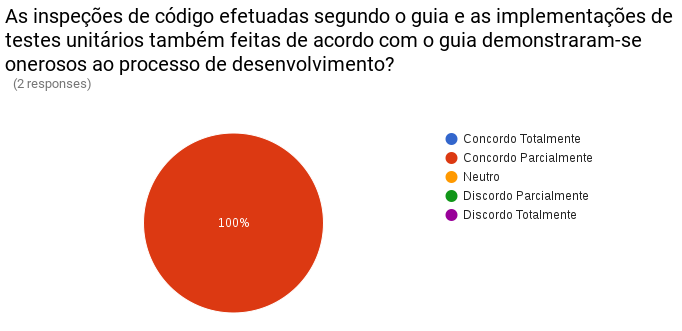
\includegraphics[width=\textwidth]{figuras/s3p.png}
\caption{Questão 3 - Satisfação dos Desenvolvedores - \textit{Sprint} 1 Portal}
\end{figure}

\begin{figure}[!h]
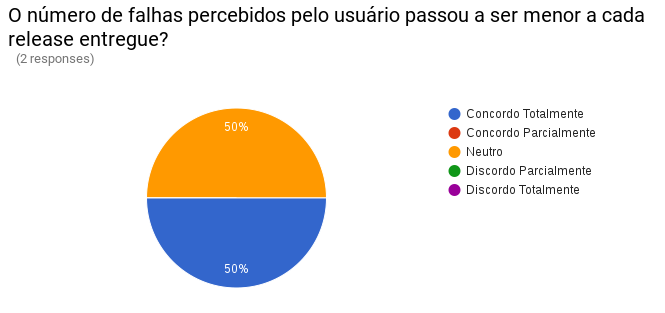
\includegraphics[width=\textwidth]{figuras/s4p.png}
\caption{Questão 4 - Satisfação dos Desenvolvedores - \textit{Sprint} 1 Portal}
\end{figure}

\begin{figure}[!h]
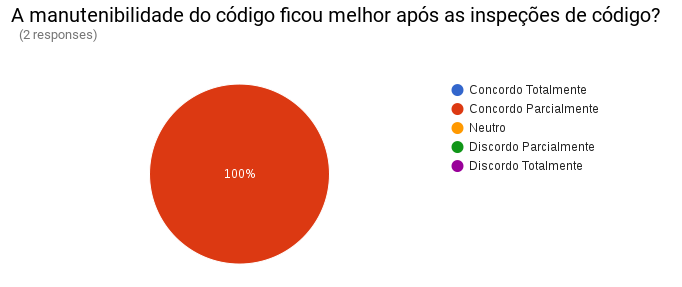
\includegraphics[width=\textwidth]{figuras/s5p.png}
\caption{Questão 5 - Satisfação dos Desenvolvedores - \textit{Sprint} 1 Portal}
\end{figure}

\clearpage

\section{\textit{Sprint} 1 - Sistema de Ouvidoria do Distrito Federal}

Assim como no projeto do portal, a primeira \textit{sprint} do projeto do sistema de ouvidoria também foi executada com êxito. A equipe de desenvolvimento também protelou as atividades de verificação, alocando-as para o final da \textit{sprint}.

A tabela a seguir exibe um resumo das métricas coletadas para as camadas de \textit{backend}.

\begin{table}[h]
\centering
\begin{tabular}{ | m{8cm} | m{8cm} | } 
\hline
Número de Defeitos & 1 \\ 
\hline
Taxa de Acertos por Linha de Código & 3 \\ 
\hline
\end{tabular}
\caption{Tabela Resumo - Métricas \textit{Sprint} 1 - Sistema de Ouvidoria (\textit{Backend})}\label{table:1}
\end{table}

A partir dos dados exibidos pela tabela, constata-se que o código foi bem implementado, tendo em vista o baixo número de defeitos identificados durante a inspeção. Adicionalmente, a suíte de testes foi capaz de exercitar, em média, 3 vezes o trecho de código sob teste.

Com relação ao índice de manutenibilidade, os valores calculados são expressos na tabela a seguir.

\begin{table}[h]
\centering
\begin{tabular}{ | m{12cm} | m{4cm} | } 
\hline
\textit{CoreAppService} - \textit{OuvCidadania.AppService} & 61 \\ 
\hline
Resposta - \textit{Domain.Entity} & 90 \\ 
\hline
Resposta Questionário - \textit{Domain.Entity} & 90 \\ 
\hline
Resposta Exception - \textit{Domain.Exceptions} & 98 \\ 
\hline
IRespostaRepository - \textit{Domain.Repository} & 100 \\
\hline
IRespostaQuestionarioService - \textit{Domain.Service} & 100 \\
\hline
IRespostaService - \textit{Domain.Service} & 100 \\
\hline
Resposta Questionario Service - \textit{Domain.Service} & 65 \\
\hline
Resposta Service - \textit{Domain.Service} & 64 \\
\hline
\end{tabular}
\caption{Índice de Manutenibilidade \textit{Sprint} 1 - Sistema de Ouvidoria (\textit{Backend})}\label{table:1}
\end{table}

Considerando os parâmetros da \textit{Microsoft}, todas as classes e interfaces apresentaram índices de manutenibilidade aceitáveis. Contudo, deve-se atentar para as classes na camada de serviço, que necessitarão de refatorações para que o índice de manutenibilidade possa aumentar.

Assim como no projeto do portal, não houve registro de falhas por parte da área de negócio. Todas as funcionalidades entregues ao final da \textit{sprint} foram estabelecidas de forma consistente.

Por fim, com relação ao índice de satisfação dos desenvolvedores, também contemplou-se uma boa percepção acerca da utilização do \textit{framework}. A equipe também considerou as práticas propostas pelo \textit{framework} onerosas para contextos de equipes pequenas e sugeriu que fosse feita uma adequação das práticas para equipes pequenas. As figuras a seguir apresentam os percentuais obtidos para cada questão do questionário de verificação da satisfação dos desenvolvedores.

\begin{figure}[!h]
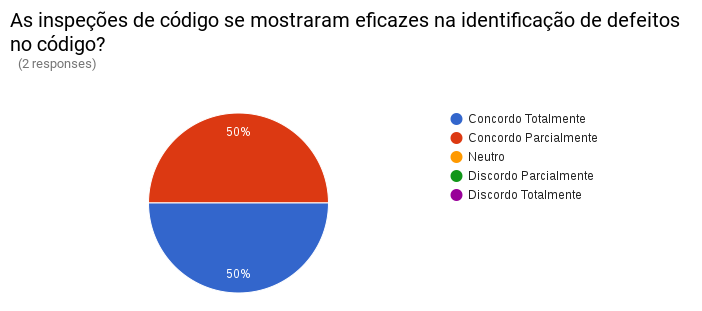
\includegraphics[width=\textwidth]{figuras/s1o.png}
\caption{Questão 1 - Satisfação dos Desenvolvedores - \textit{Sprint} 1 Ouvidoria}
\end{figure}

\begin{figure}[!h]
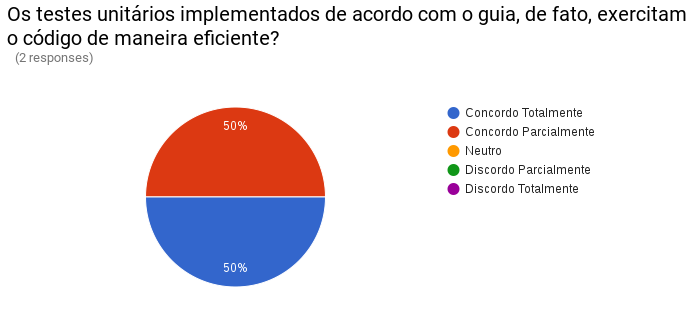
\includegraphics[width=\textwidth]{figuras/s2o.png}
\caption{Questão 2 - Satisfação dos Desenvolvedores - \textit{Sprint} 1 Ouvidoria}
\end{figure}

\begin{figure}[!h]
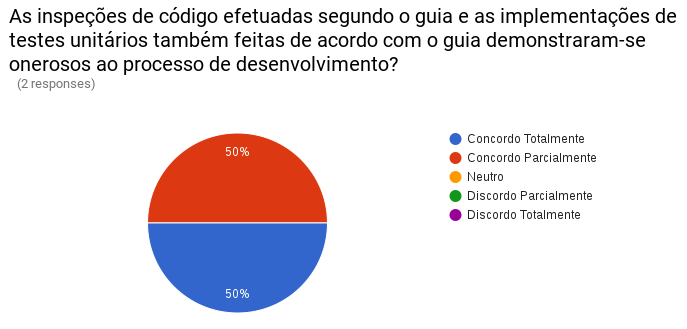
\includegraphics[width=\textwidth]{figuras/s3o.png}
\caption{Questão 3 - Satisfação dos Desenvolvedores - \textit{Sprint} 1 Ouvidoria}
\end{figure}

\begin{figure}[!h]
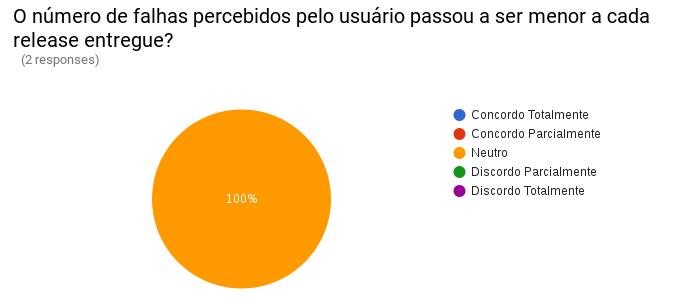
\includegraphics[width=\textwidth]{figuras/s4o.png}
\caption{Questão 4 - Satisfação dos Desenvolvedores - \textit{Sprint} 1 Ouvidoria}
\end{figure}

\begin{figure}[!h]
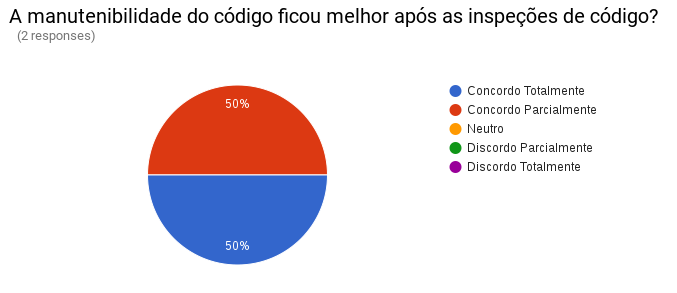
\includegraphics[width=\textwidth]{figuras/s5o.png}
\caption{Questão 5 - Satisfação dos Desenvolvedores - \textit{Sprint} 1 Ouvidoria}
\end{figure}